\PassOptionsToPackage{unicode=true}{hyperref} % options for packages loaded elsewhere
\PassOptionsToPackage{hyphens}{url}
%
\documentclass[ignorenonframetext,aspectratio=169,12pt]{beamer}
\usepackage{pgfpages}
\setbeamertemplate{caption}[numbered]
\setbeamertemplate{caption label separator}{: }
\setbeamercolor{caption name}{fg=normal text.fg}
\beamertemplatenavigationsymbolsempty
\usepackage{lmodern}
\usepackage{amssymb,amsmath}
\usepackage{ifxetex,ifluatex}
\usepackage{fixltx2e} % provides \textsubscript
\ifnum 0\ifxetex 1\fi\ifluatex 1\fi=0 % if pdftex
  \usepackage[T1]{fontenc}
  \usepackage[utf8]{inputenc}
  \usepackage{textcomp} % provides euro and other symbols
\else % if luatex or xelatex
  \usepackage{unicode-math}
  \defaultfontfeatures{Ligatures=TeX,Scale=MatchLowercase}
\fi
% use upquote if available, for straight quotes in verbatim environments
\IfFileExists{upquote.sty}{\usepackage{upquote}}{}
% use microtype if available
\IfFileExists{microtype.sty}{%
\usepackage[]{microtype}
\UseMicrotypeSet[protrusion]{basicmath} % disable protrusion for tt fonts
}{}
\IfFileExists{parskip.sty}{%
\usepackage{parskip}
}{% else
\setlength{\parindent}{0pt}
\setlength{\parskip}{6pt plus 2pt minus 1pt}
}
\usepackage{hyperref}
\hypersetup{
            pdfborder={0 0 0},
            breaklinks=true}
\urlstyle{same}  % don't use monospace font for urls
\newif\ifbibliography
% Prevent slide breaks in the middle of a paragraph:
\widowpenalties 1 10000
\raggedbottom
\setbeamertemplate{part page}{
\centering
\begin{beamercolorbox}[sep=16pt,center]{part title}
  \usebeamerfont{part title}\insertpart\par
\end{beamercolorbox}
}
\setbeamertemplate{section page}{
\centering
\begin{beamercolorbox}[sep=12pt,center]{part title}
  \usebeamerfont{section title}\insertsection\par
\end{beamercolorbox}
}
\setbeamertemplate{subsection page}{
\centering
\begin{beamercolorbox}[sep=8pt,center]{part title}
  \usebeamerfont{subsection title}\insertsubsection\par
\end{beamercolorbox}
}
\AtBeginPart{
  \frame{\partpage}
}
\AtBeginSection{
  \ifbibliography
  \else
    \frame{\sectionpage}
  \fi
}
\AtBeginSubsection{
  \frame{\subsectionpage}
}
\setlength{\emergencystretch}{3em}  % prevent overfull lines
\providecommand{\tightlist}{%
  \setlength{\itemsep}{0pt}\setlength{\parskip}{0pt}}
\setcounter{secnumdepth}{0}

% set default figure placement to htbp
\makeatletter
\def\fps@figure{htbp}
\makeatother

\DeclareUnicodeCharacter{00A0}{~}
\DeclareUnicodeCharacter{03B4}{$\delta$}
\DeclareUnicodeCharacter{03B5}{$\varepsilon$}
\DeclareUnicodeCharacter{03C9}{$\omega$}
\DeclareUnicodeCharacter{2124}{\mathbb{Z}}
\DeclareUnicodeCharacter{2193}{$\downarrow$}
\DeclareUnicodeCharacter{2208}{$\in$}
\DeclareUnicodeCharacter{2209}{$\notin$}
\DeclareUnicodeCharacter{220B}{$\ni$}
\DeclareUnicodeCharacter{2227}{$\wedge$}
\DeclareUnicodeCharacter{2228}{$\vee$}
\DeclareUnicodeCharacter{2234}{$\therefore$}
\DeclareUnicodeCharacter{2264}{$\leq$}
\DeclareUnicodeCharacter{2265}{$\geq$}
\DeclareUnicodeCharacter{2605}{$\star$}
\DeclareUnicodeCharacter{1D53D}{\mathbb{F}}

% Scale images if necessary, so that they will not overflow the page
% margins by default, and it is still possible to overwrite the defaults
% using explicit options in \includegraphics[width, height, ...]{}
%\setkeys{Gin}{width=\maxwidth,height=\maxheight,keepaspectratio}
\newcommand{\includegraphicsscaled}[1]{
    \includegraphics[width=\maxwidth,height=\maxheight,keepaspectratio]{#1}
}


\hypersetup{colorlinks,linkcolor=,urlcolor=purple}
\setbeamertemplate{navigation symbols}{}
\usefonttheme[onlymath]{serif}

\setbeamercolor{footnote mark}{fg=gray}
\setbeamerfont{footnote}{size=\tiny}
\usepackage{color}
\usepackage[normalem]{ulem}
\usepackage{listings}
\lstset{
    basicstyle=\ttfamily\normalsize,
    keywordstyle=\color{blue}\bfseries,
    commentstyle=\color[rgb]{0,0.5,0}\bfseries\em,
    stringstyle=\color{red}\bfseries\em,
    escapeinside={(*}{*)}
}

\usepackage{graphicx,grffile}
\makeatletter
\def\maxwidth{\ifdim\Gin@nat@width>\linewidth\linewidth\else\Gin@nat@width\fi}
\def\maxheight{\ifdim\Gin@nat@height>\textheight\textheight\else\Gin@nat@height\fi}
\makeatother

\title{\bf Security response for open source ecosystems}
\author{{\bf Fraser Tweedale}\\
    \texttt{@hackuador[@functional.cafe]}}
\date{2025-03-22}

\begin{document}
\frame{
  \titlepage
\centering

\includegraphics[height=0.4\maxheight]{qr.png}
}


%\section{Why open source security matters}


\begin{frame}[plain]
\begin{center}
    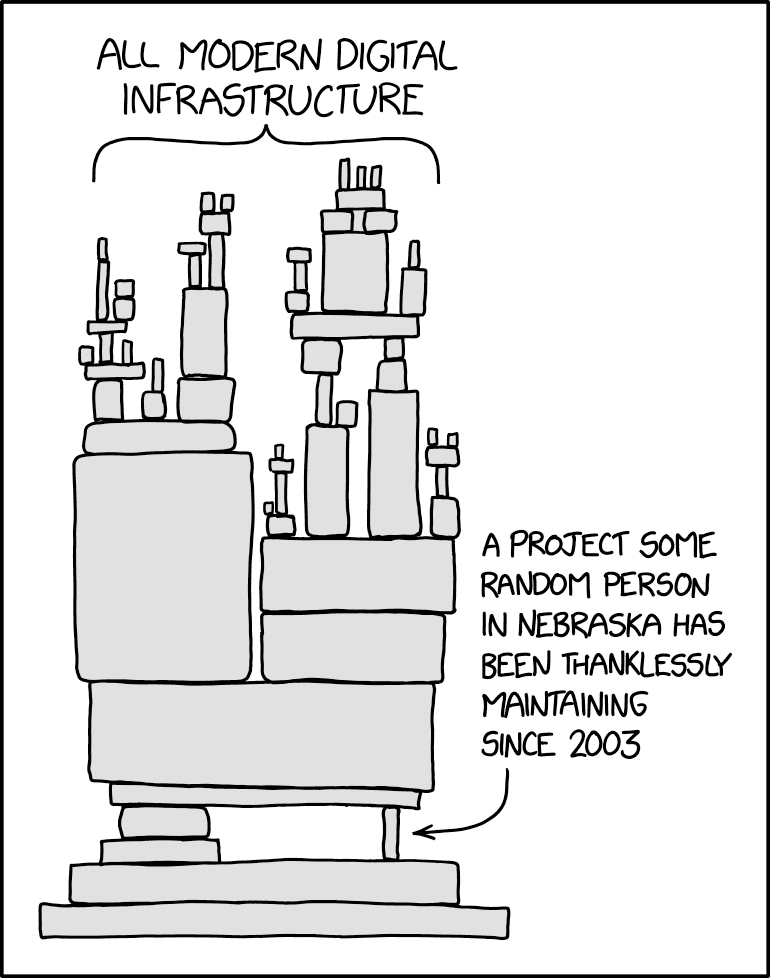
\includegraphics[height=0.9\maxheight,keepaspectratio]{dependency_2x.png}
    \\
    \tiny
    CC-BY-NC 2.5 \texttt{\url{https://xkcd.com/2347/}}
\end{center}
\end{frame}

\begin{frame}{Why open source security matters}
    \begin{itemize}
        \item supply chain security
        \item ISO 27001 de-risking
        \item NIST SP 800-218 (SSDF)
            \footnote{\url{https://csrc.nist.gov/pubs/sp/800/218/final}}
            + EO 14028 (procurement)
            \footnote{\url{https://www.nist.gov/system/files/documents/2022/02/04/software-supply-chain-security-guidance-under-EO-14028-section-4e.pdf}}
        \item EU Cyber Resilience Act
            \footnote{\url{https://eur-lex.europa.eu/legal-content/EN/TXT/HTML/?uri=OJ:L_202402847&qid=1732732976975\#art_24}}
            \footnote{\url{https://github.blog/open-source/maintainers/what-the-eus-new-software-legislation-means-for-developers/}}
    \end{itemize}
\end{frame}

\begin{frame}{Why open source security matters}
\begin{quote}
\raggedright
  Open-source software {stewards} shall put in place\ldots{}
  a {cybersecurity policy} to foster\ldots{}
  effective {handling of vulnerabilities}\ldots{}
  also foster the {voluntary reporting} of vulnerabilities\ldots{}
  promote the {sharing of information} concerning discovered vulnerabilities
\\
  {\hfill --- \footnotesize Cyber Resilience Act, Article 24 {\em
  \textbf{Obligations of open-source software stewards}}}
\end{quote}
\end{frame}

\begin{frame}{Why open source security matters}
\large
\begin{quote}
\raggedright
Supply chain security has always been important.  But market
  participants and open source organisations care more now (because
  they've been forced to).

\bigskip

Therefore, open source projects and ecosystems that lack an
effective security apparatus will be left behind.
\end{quote}
\end{frame}

\begin{frame}{Who needs a security response apparatus?}
    \begin{itemize}
        \item operating systems
        \item programming languages + library ecosystems
        \item frameworks
        \item applications + network servers
        \item other large projects
    \end{itemize}
\end{frame}

\begin{frame}{Haskell Security Response Team (SRT)}
  \begin{itemize}
    \item Haskell Foundation {\em tech proposal}
          \footnote{\url{https://github.com/haskellfoundation/tech-proposals/blob/main/proposals/accepted/037-advisory-db.md}}
    \item Fraser was asked to recruit and lead the team
  \end{itemize}
\end{frame}


\section{How to build a security response team}

\begin{frame}{Building a team - skills}
    \begin{itemize}
        \item technical skills / knowledge of the language / project
        \item security know-how: AppSec, IR, GRC, pen
          testing, IAM, vuln research, \ldots{}
        \item programming ability (for tool development)
        \item good communication skills
    \end{itemize}
\end{frame}

\begin{frame}{Building a team - how many?}
    \begin{itemize}
        \item enough to cover the skills you want / need
        \item enough to tolerate absences
        \item {\bf not all} the qualified people all at once
        \item diversity is good!
        \item {\em Haskell: 5 $\to$ 6 people}
    \end{itemize}
\end{frame}

\begin{frame}{Defining the scope of work}
  \begin{itemize}
    \item triage security reports
      \begin{itemize}
        \item analyse reports and propose action
        \item coordinate with maintainers and stakeholders
      \end{itemize}
    \item publish advisories
    \item oversee project infrastructure security
    \item developer tooling
    \item reports, guides, documentation, \ldots{}
  \end{itemize}

  You can't do everything.  Choose a scope and review it regularly.
\end{frame}

\begin{frame}{Building a team - call for volunteers}
  \begin{itemize}
    \item preamble
    \item team responsibilities
    \item desired skills / experience
    \item how to apply
    \item {\em Haskell SRT example}\footnote{\url{https://github.com/haskell/security-advisories/blob/main/docs/call-for-volunteers-example.md}} (feel free to copy!)
  \end{itemize}
\end{frame}

\begin{frame}{Processes and communication}
    \begin{itemize}
        \item reporting and disclosure processes
        \item team chat / mailing list (private!)
        \item meetings ({\em Haskell: every 2 weeks})
        \item activity reports ({\em Haskell: quarterly})
        \item community engagement (conferences, discussions, office hours)
    \end{itemize}
\end{frame}


\section{Security advisories and tooling}

\begin{frame}{Advisory naming}
  \begin{itemize}
    \item some ecosystems/projects use own namespace
      (e.g. {\em HSEC-YYYY-NNNN})
    \item some are a CVE Numbering Authority (CNA)
        \footnote{\url{https://github.com/ossf/wg-vulnerability-disclosures/blob/main/docs/guides/becoming-a-cna-as-an-open-source-org-or-project.md}}
      \begin{itemize}
        \item {\bf suppress bogus CVEs}
          \footnote{\url{https://lwn.net/Articles/961978/}}
        \item produce higher-quality CVE records
      \end{itemize}
    \item some use existing CNAs
  \end{itemize}
\end{frame}

\begin{frame}{Advisory content}
  \begin{itemize}
    \item description (give detail!)
    \item affected packages and versions
    \item CVSS, CWE
    \item aliases and related IDs
    \item references (reports, PoC, commits, \ldots{})
  \end{itemize}
\end{frame}


\begin{frame}[fragile]
\scriptsize
\begin{verbatim}
```toml
[advisory]
id = "HSEC-2023-0001"
cwe = [328, 400]
keywords = ["json", "dos", "historical"]
aliases = ["CVE-2022-3433"]

[[affected]]
package = "aeson"
cvss = "CVSS:3.1/AV:N/AC:L/PR:L/UI:N/S:U/C:N/I:N/A:H"

[[affected.versions]]
introduced = "0.4.0.0"
fixed = "2.0.1.0"
```

# Hash flooding vulnerability in aeson

*aeson* was vulnerable to hash flooding (a.k.a. hash DoS).  The
issue is a consequence of the HashMap implementation from
*unordered-containers*.  It results in a denial of service through
CPU consumption.  This technique has been used in real-world attacks
against a variety of languages, libraries and frameworks over the
years.

\end{verbatim}
\end{frame}

\begin{frame}{Advisory database - outputs}
  \begin{itemize}
    \item OSV (ingested by
      osv.dev\footnote{\url{https://osv.dev/list?ecosystem=Hackage}})
    \item HTML index\footnote{\url{https://haskell.github.io/security-advisories/}}
    \item "snapshot" format (for downstream tooling)
  \end{itemize}
\end{frame}

\begin{frame}{osv.dev}
  \begin{itemize}
    \item \texttt{\url{https://osv.dev/}}
    \item aggregates many advisory databases
    \item JSON schema\footnote{\url{https://github.com/ossf/osv-schema}}
    \item to integrate your advisories:
      \begin{itemize}
        \item publish your osv json somewhere
        \item ask osv.dev to ingest it (GitHub issue)
        \item they might need a bit of info or help
    \end{itemize}
  \end{itemize}
\end{frame}

\begin{frame}{Package repositories}
  \begin{itemize}
    \item e.g. PyPI, npm, Maven, \ldots{}
    \item integrate advisory info in package pages
    \item link to advisories
    \item reporting mechanism / info
  \end{itemize}
\end{frame}

\begin{frame}{Audit tooling}
  \begin{itemize}
    \item check build plans or lock files for vulnerable dependencies
    \item call analysis (advanced; not always feasible)
    \item {\tt osv-scanner}\footnote{\url{https://google.github.io/osv-scanner/}}
      is a good starting point
  \end{itemize}
\end{frame}

\begin{frame}{Exploitability information}
  \begin{itemize}
    \item suppress false positives
    \item VEX - {\em Vulnerability Exploitability
      eXchange}\footnote{\url{https://www.cisa.gov/resources-tools/resources/minimum-requirements-vulnerability-exploitability-exchange-vex}}
      \begin{itemize}
        \item statements that dependency issue is(n't) exploitable
        \item {\bf data model} by CISA.gov, several implementations
        %\item implementations:
        % \href{https://github.com/openvex/spec}{OpenVEX},
        % \href{https://spdx.dev/capturing-software-vulnerability-data-in-spdx-3-0/}{SPDX 3.0},
        % \href{https://www.oasis-open.org/2022/11/21/new-version-of-csaf-standard/}{OASIS CSAF 2.0},
        % CycloneDX 
      \end{itemize}
    \item produce, collect, distribute
    \item advisory DB as a VEX clearing-house?
  \end{itemize}
\end{frame}

\begin{frame}{Advisory data in aggregate}
  \begin{itemize}
    \item what kinds of issues commonly arise in your ecosystem?
      \begin{itemize}
        \item improve developer practices
        \item improve detection mechanisms
      \end{itemize}
    \item identify problematic packages / authors / abandonware
      \begin{itemize}
        \item make {\em tribal knowledge} explicit
        \item can policy or technical controls help? (nuance!)
      \end{itemize}
    \item corollary: {\bf historical advisories} are important
  \end{itemize}
\end{frame}

\begin{frame}{Embargoed advisories}
  \begin{itemize}
    \item what threshold for embargo? (you decide)
    \item notifying downstream {\bf redistributors} (e.g. Linux distros)
    \item multi-ecosystem vulnerabilities
    \item {\em Vulnerability Information and Coordination
      Environment (VINCE)}\footnote{\url{https://kb.cert.org/vince/}}
      \begin{itemize}
        \item enable secure reporting and cross-vendor collab
        \item register your project / ecosystem!
      \end{itemize}
  \end{itemize}
\end{frame}

\begin{frame}{Bug bounties and audits}
  \begin{itemize}
    \item if you can fund them, great
    \item fund security response capacity first!
  \end{itemize}
\end{frame}




\section{Sustainability}

\begin{frame}{A not good scenario}
  \begin{itemize}
    \item critical issue disclosed
    \item requires significant effort and coordination
    \item everyone is busy with their day job and life
    \item issue remains unfixed\ldots{}
  \end{itemize}
\end{frame}

\begin{frame}{Bottom line}
\large
\begin{quote}
\raggedright
  Open source ecosystems need personnel with {\bf capacity} and
  {\bf authority} to respond {\bf immediately} to security incidents.
\end{quote}
\end{frame}

\begin{frame}{Things that don't work}
  \begin{itemize}
    \item empty words of support
    \item burying your head in the sand
    \item a few thousand dollaridoos here and there
    \item thoughts and prayers
  \end{itemize}
\end{frame}

\begin{frame}{Models I have observed}
  \begin{itemize}
    \item company employees doing security work (full- or part-time)
    \item foundation-funded {\em security officer} role
    \item foundation-funded ad-hoc projects (e.g. audits, tooling)
    \item grants for bounties or ad-hoc projects (e.g.
      EU-FOSSA\footnote{\url{https://commission.europa.eu/about/departments-and-executive-agencies/digital-services/eu-fossa-2-free-and-open-source-software-auditing_en}},
      GitHub\footnote{GitHub Secure Open Source Fund:
      \url{https://resources.github.com/github-secure-open-source-fund/}},
      Sovereign Tech
      Fund\footnote{\url{https://nkcs.bund.de/en/news/renewed-general-financing-sovereign-tech-fund}})
    \item all-volunteer effort ({\em $\gets$ Haskell is here})
  \end{itemize}
\end{frame}

\begin{frame}{Things that might work?}
  \begin{itemize}
    \item volunteer team with paid lead {\em (awkard?)}
    \item paid worker with diverse assignments including IR (which has
      priority)
  \end{itemize}
\end{frame}

\begin{frame}{How to get money}
  \begin{itemize}
    \item grants
    \item foundation funding
      \begin{itemize}
        \item big enough for a foundation $\to$ fund security work
      \end{itemize}
    \item subscription program
      \begin{itemize}
        \item commercial users directly fund security work; in
          return you get…
          \begin{itemize}
            \item a heads-up on active issues
            \item a say in priorities, tooling
            \item access to team for advice/consulting
          \end{itemize}
      \end{itemize}
  \end{itemize}
\end{frame}


\begin{frame}{Moral obligations of F/OSS users}
\large
\begin{quote}
\raggedright
We estimate the supply-side value of widely-used OSS is \$4.15
billion, but that the demand-side value is much larger at {\bf \$8.8
trillion}. We find that {\bf firms would need to spend 3.5 times more} on
software than they currently do if OSS did not exist.\\
{\hfill --- \small The Value of Open Source Software, Harvard Business
School 2024\footnote{\url{
  https://www.hbs.edu/faculty/Pages/item.aspx?num=65230
}}}
\end{quote}
\end{frame}

\begin{frame}{Moral obligations of F/OSS users}
\large
\raggedright
If you depend on F/OSS ecosystems, you SHOULD contribute
to the security of those ecosystems.

\bigskip

If you are impacted by security issues in F/OSS ecosystems,
but did not contribute to the security of those ecosystems,
you SHALL NOT complain.

\bigskip

If you are the government, funding F/OSS security work
  through grants is RECOMMENDED.
\end{frame}


\begin{frame}{Moral obligations of F/OSS {\bf authors}}
\large
\raggedright
Reasonable effort not to deliver insecure code, and reasonable
effort to fix discovered issues.

\bigskip

What is {\em reasonable} depends on the level of financial or in-kind
support the developers receive in respect of the affected component.
\end{frame}



\section{Conclusion}

\begin{frame}{What we discussed}
  \begin{itemize}
    \item why open source security response matters
    \item how to bootstrap and run a security team
    \item advisories and related tooling
    \item sustainability and funding
  \end{itemize}
\end{frame}


% END MATTER

\begin{frame}[plain]
\begin{columns}

  \begin{column}{.4\textwidth}
    \begin{center}
    {
        {\Large \textsc{Thank you}}

        \bigskip

        This slide deck:\\
        \includegraphicsscaled{qr.png}
    }
    \end{center}
  \end{column}

  \begin{column}{.6\textwidth}

    \setlength{\parskip}{.5em}

    { \centering

    \input{cc-by-ARTIFACT.pdf_tex}

    \copyright~2025  Fraser Tweedale

    { \scriptsize
    Except where otherwise noted this work is licensed under
    }
    { \footnotesize
    \textbf{http://creativecommons.org/licenses/by/4.0/}
    }

    }

    \begin{description}
      \small
      \item[Socials]
        \href{https://functional.cafe/@hackuador}{@hackuador[@functional.cafe]}
      \item[Haskell SRT] \url{https://www.haskell.org/security/}
    \end{description}
  \end{column}

\end{columns}
\end{frame}

\end{document}
